\subsection{29 августа. Д.р. Кубань}
\textit{Метеоусловия: утром, днём ясно, жарко. Вечером~-- переменная облачность}

\begin{figure}[h!]
	\centering
	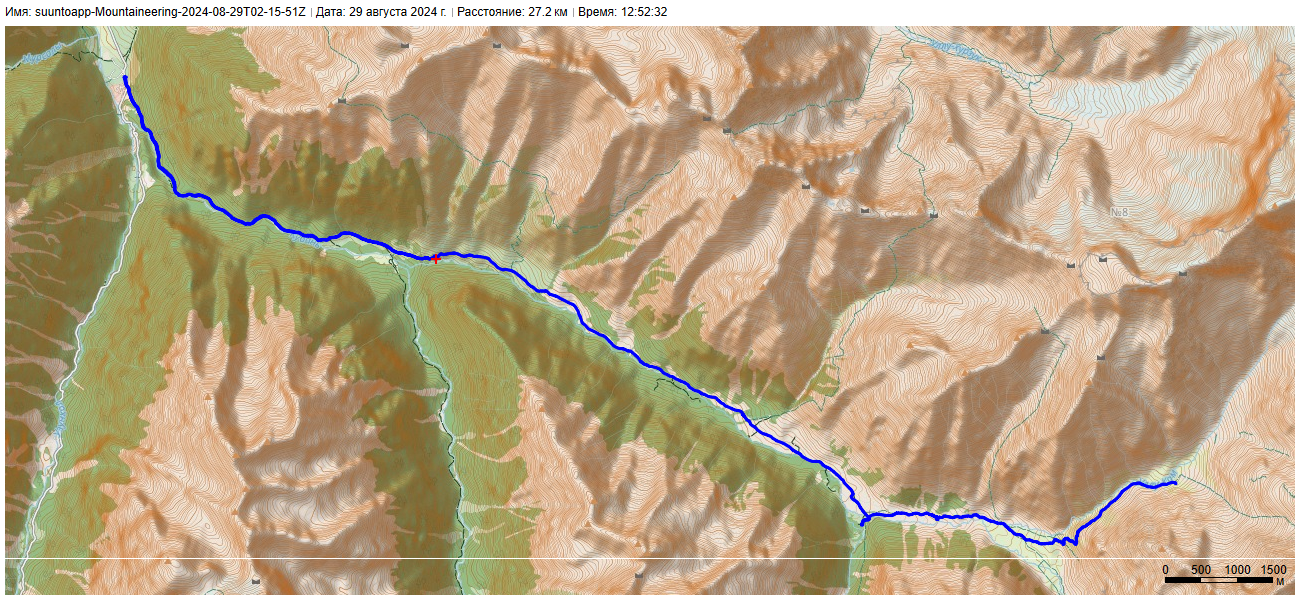
\includegraphics[angle=0, width=0.7\linewidth]{../pics/mini_maps/29}
	\label{fig:mini_29}
\end{figure}


Подъём руководов и части группы, которая сходит с маршрута (Дима Сингалевич, Илья, Даша Мерзликина, Маша), в 04:30. В 05:16 вышли вниз по д.р. Кубань. В 06:35 подошли к погранзаставе Актюбе-Хурзук. Необходимость сопровождения группы была обусловлена не только безопасностью, но и тем, что был оформлен групповой пропуск, и без заявителя группа не смогла бы покинуть погранзону. По пути обращали на себя внимание синие метки --- как выяснилось позже, трейлраннинговой тропы <<Alpindistria Elbrus Race>>.

В 08:30 руководитель и замруководителя вернулись в лагерь, где оставшаяся часть группы покормила их завтраком. Группа в текущем составе вышла вверх по д.р. Кубань в 10:00.


Шли по хорошей автомобильной грунтовой дороге практически без набора высоты. Дорога здесь идёт по открытой местности, иногда сменяется лесом. Стояла жара, у ручьёв делали привалы и набирали воду. Слева пхд тянулись каменные руины, предположительно, древних городищ.


В 12:50 дошли до Ворошиловских кошей, откуда свернули направо пхд, к погранзаставе. Прождали пограничников 15 минут, и даже пробовали им покричать, но никто не откликнулся и не вышел. Пройдя немногим более 1~км вверх по течению р. Кубань, встали на обед в 13:40 около небольшого ручья в тени деревьев, координаты места обеда N43.298154\degree,~E42.333682\degree. Во время нашего обеда к нам всё-таки подошли два конных пограничника и поинтересовались нашим маршрутом, но документов не спрашивали.

С обеда выдвинулись в 15:20 в сторону ущелья Уллу-Кам; ориентировались, кроме всего прочего, на синие метки трейраннинговой тропы.

\begin{figure}[h!]
	\centering
	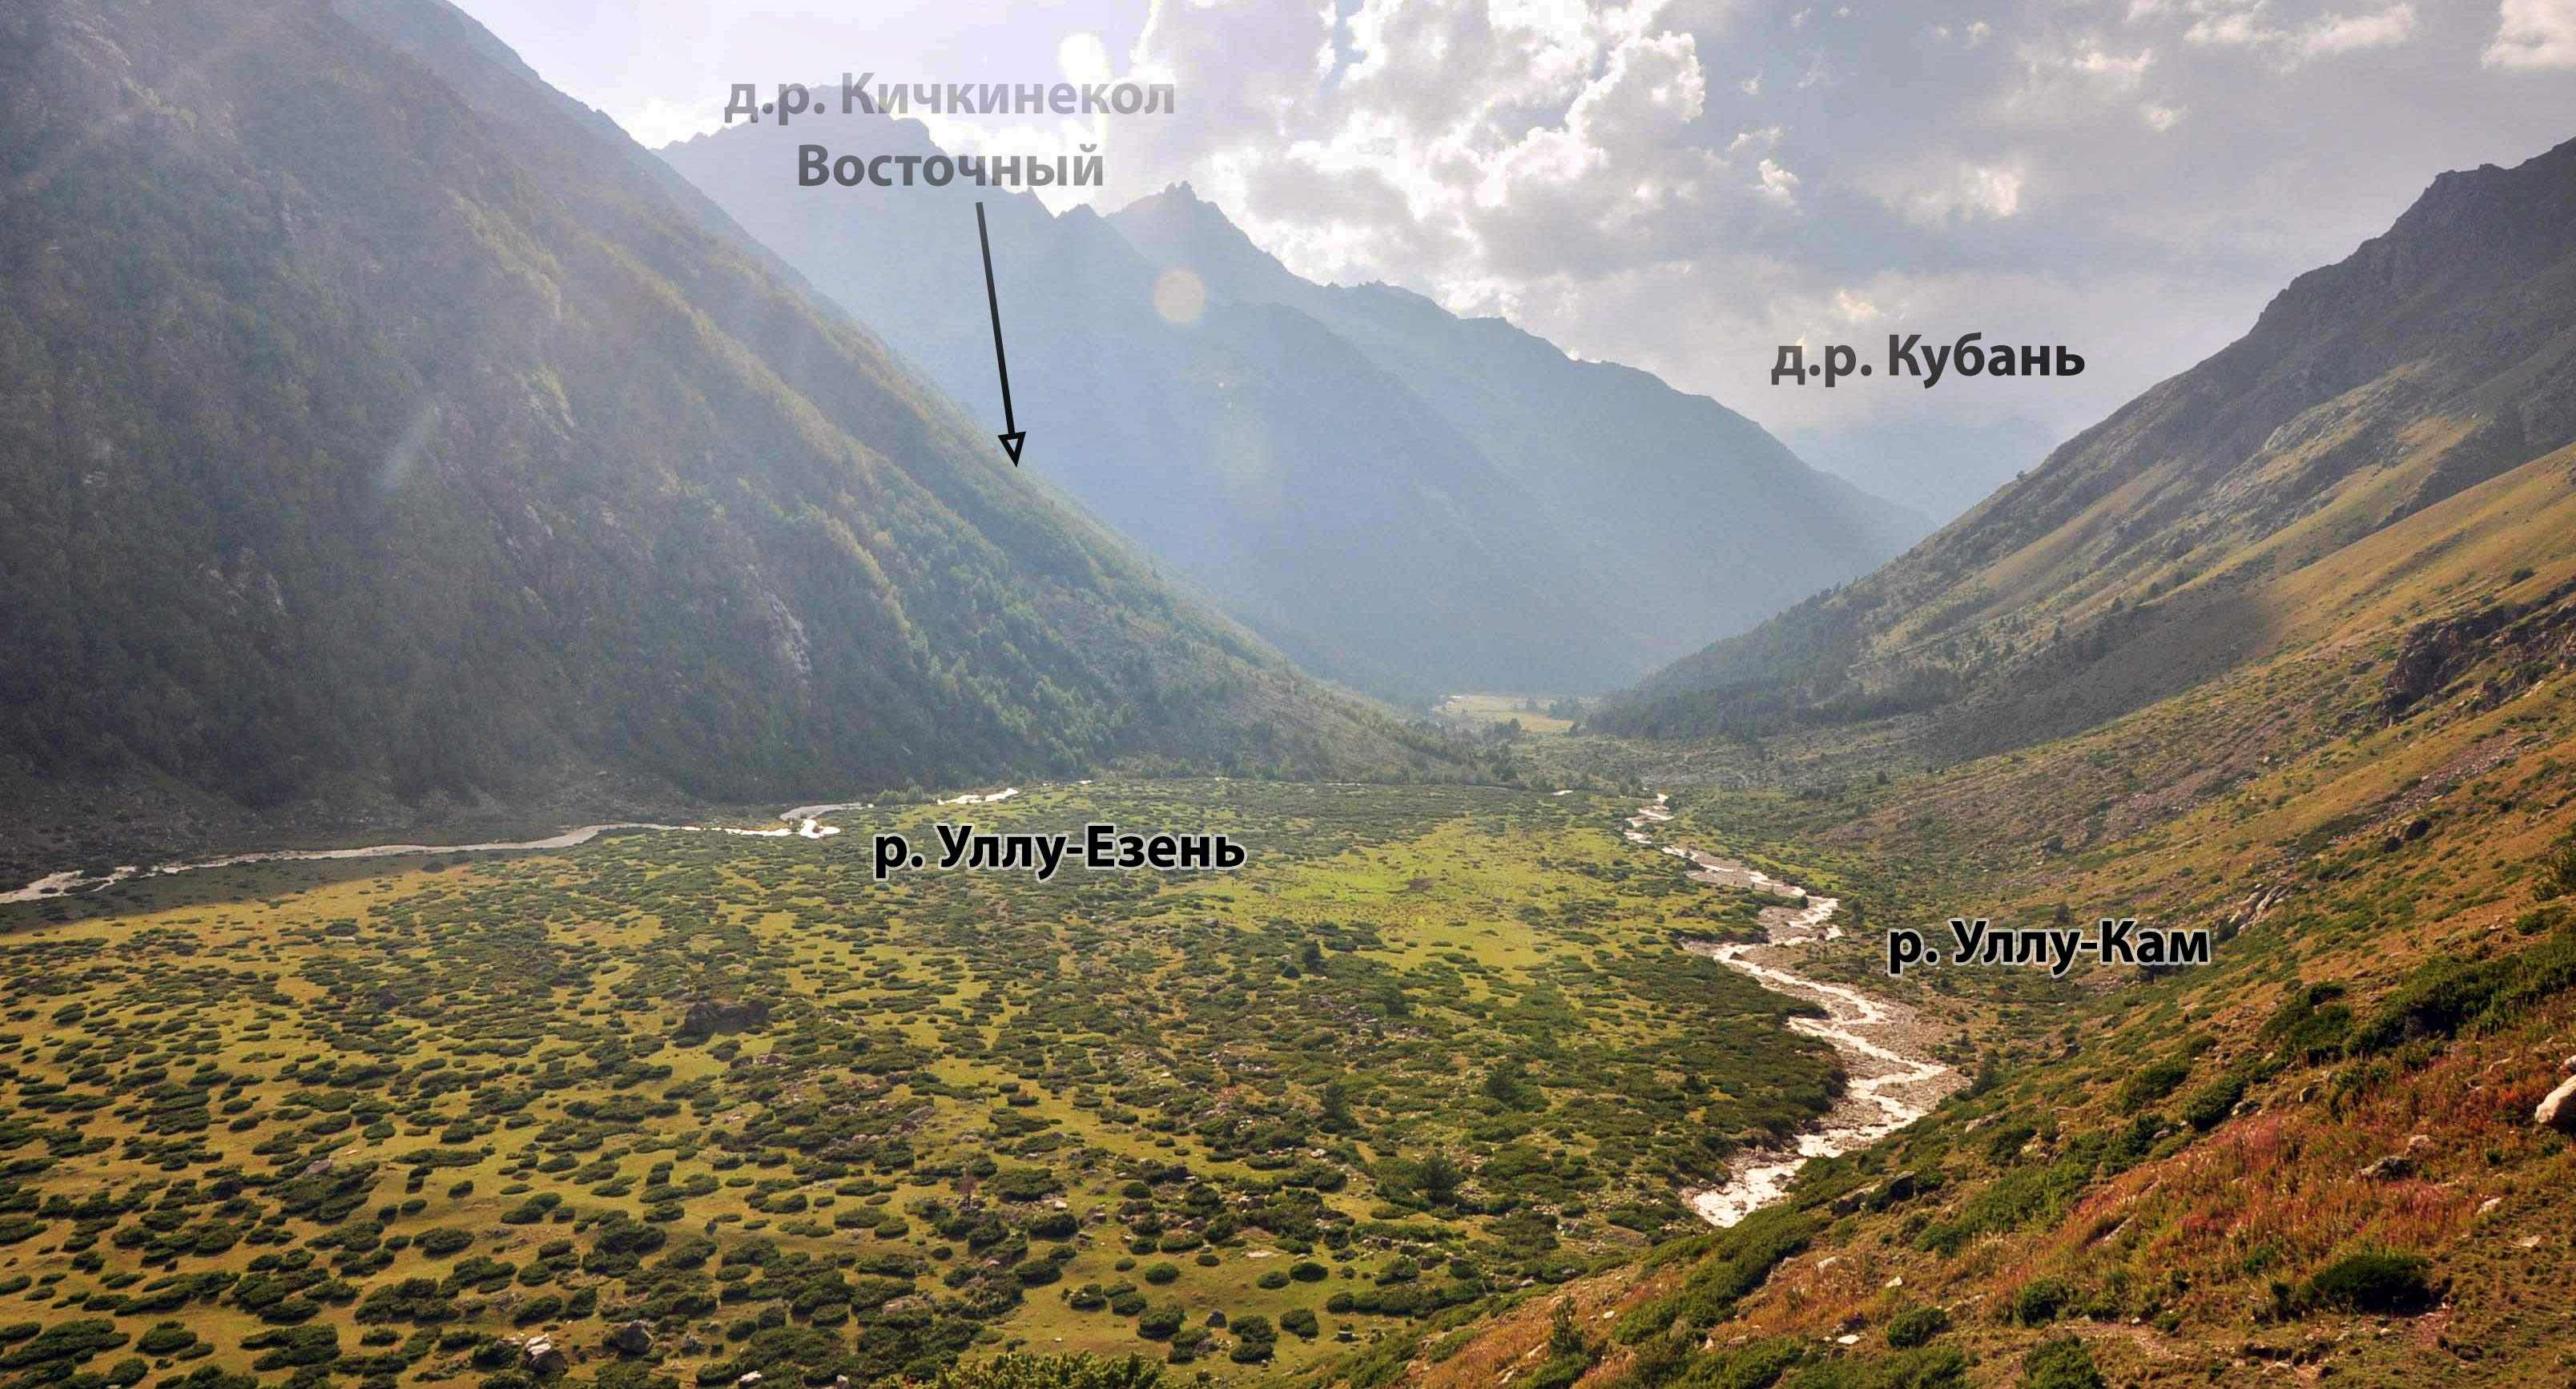
\includegraphics[width=0.7\linewidth]{../pics/DSC_0464 2.JPG}
	\caption{д.р. Кубань, вид с подъёма в д.р. Уллу-Кам}
	\label{fig:DSC_0464 2.JPG}
\end{figure}

После прохождения разлива рек Уллу-Кам (<<Кам>>~--- реликт алано-осетннской топонимии Карачая, имеется в виду <<Большая долина>> \cite{proza})и Уллу-Езень (карач.-балк. <<Большая долина>>) повернули налево пхд в ущелье Уллу-Кам. Подъём в висячую долину р. Уллу-Кам начали в 16:20. Тропа здесь идёт по левому берегу реки, резко уходя вверх, затем пологим траверсом, выходя к берегу у оборудованного места ночёвки.


\begin{figure}[h!]
	\centering
	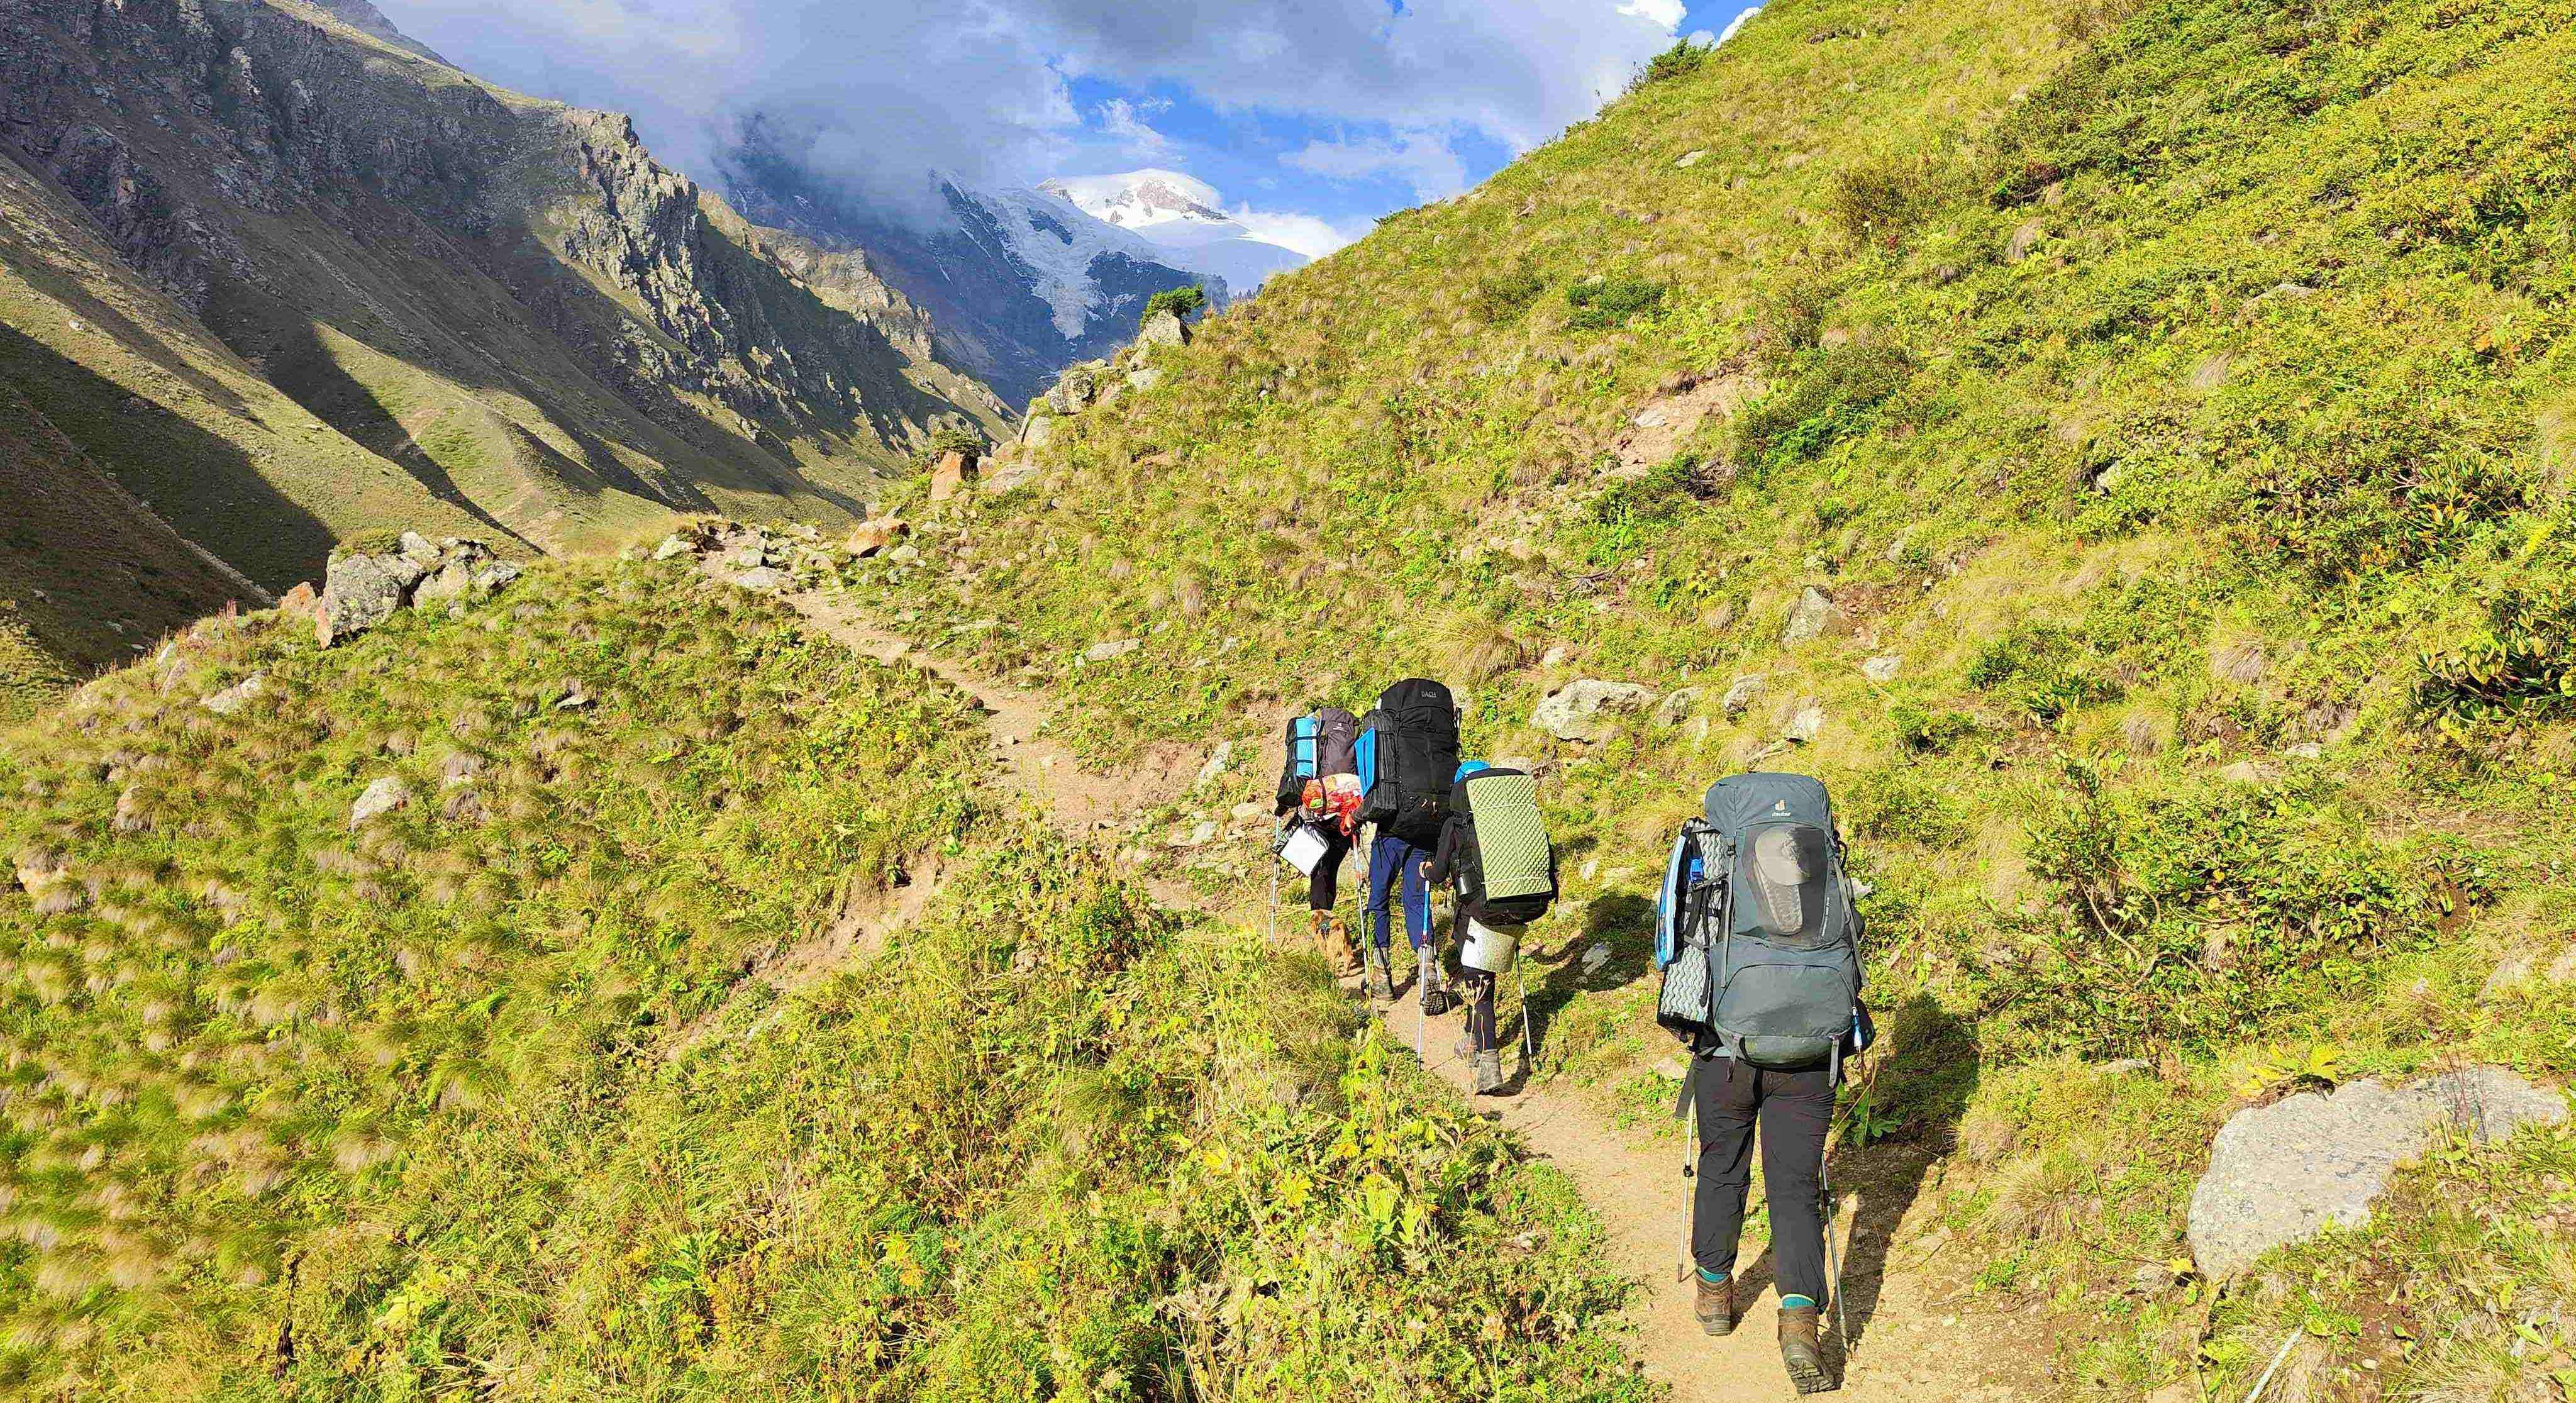
\includegraphics[width=0.7\linewidth]{../pics/IMG_20240829_170756.jpg}
	\caption{Тропа по траверсу}
	\label{fig:IMG_20240829_170756.jpg}
\end{figure}

За одним из поворотов нам открылся вид на юго-восточные скалы Эльбруса. Зрелище было завораживающим: на переднем плане простираются травяные горные склоны, на среднем плане они резко сменяются башнями Эльбруса из красной вулканической породы, а на дальнем плане~--- величественные снежные склоны.

\begin{figure}[h!]
	\centering
	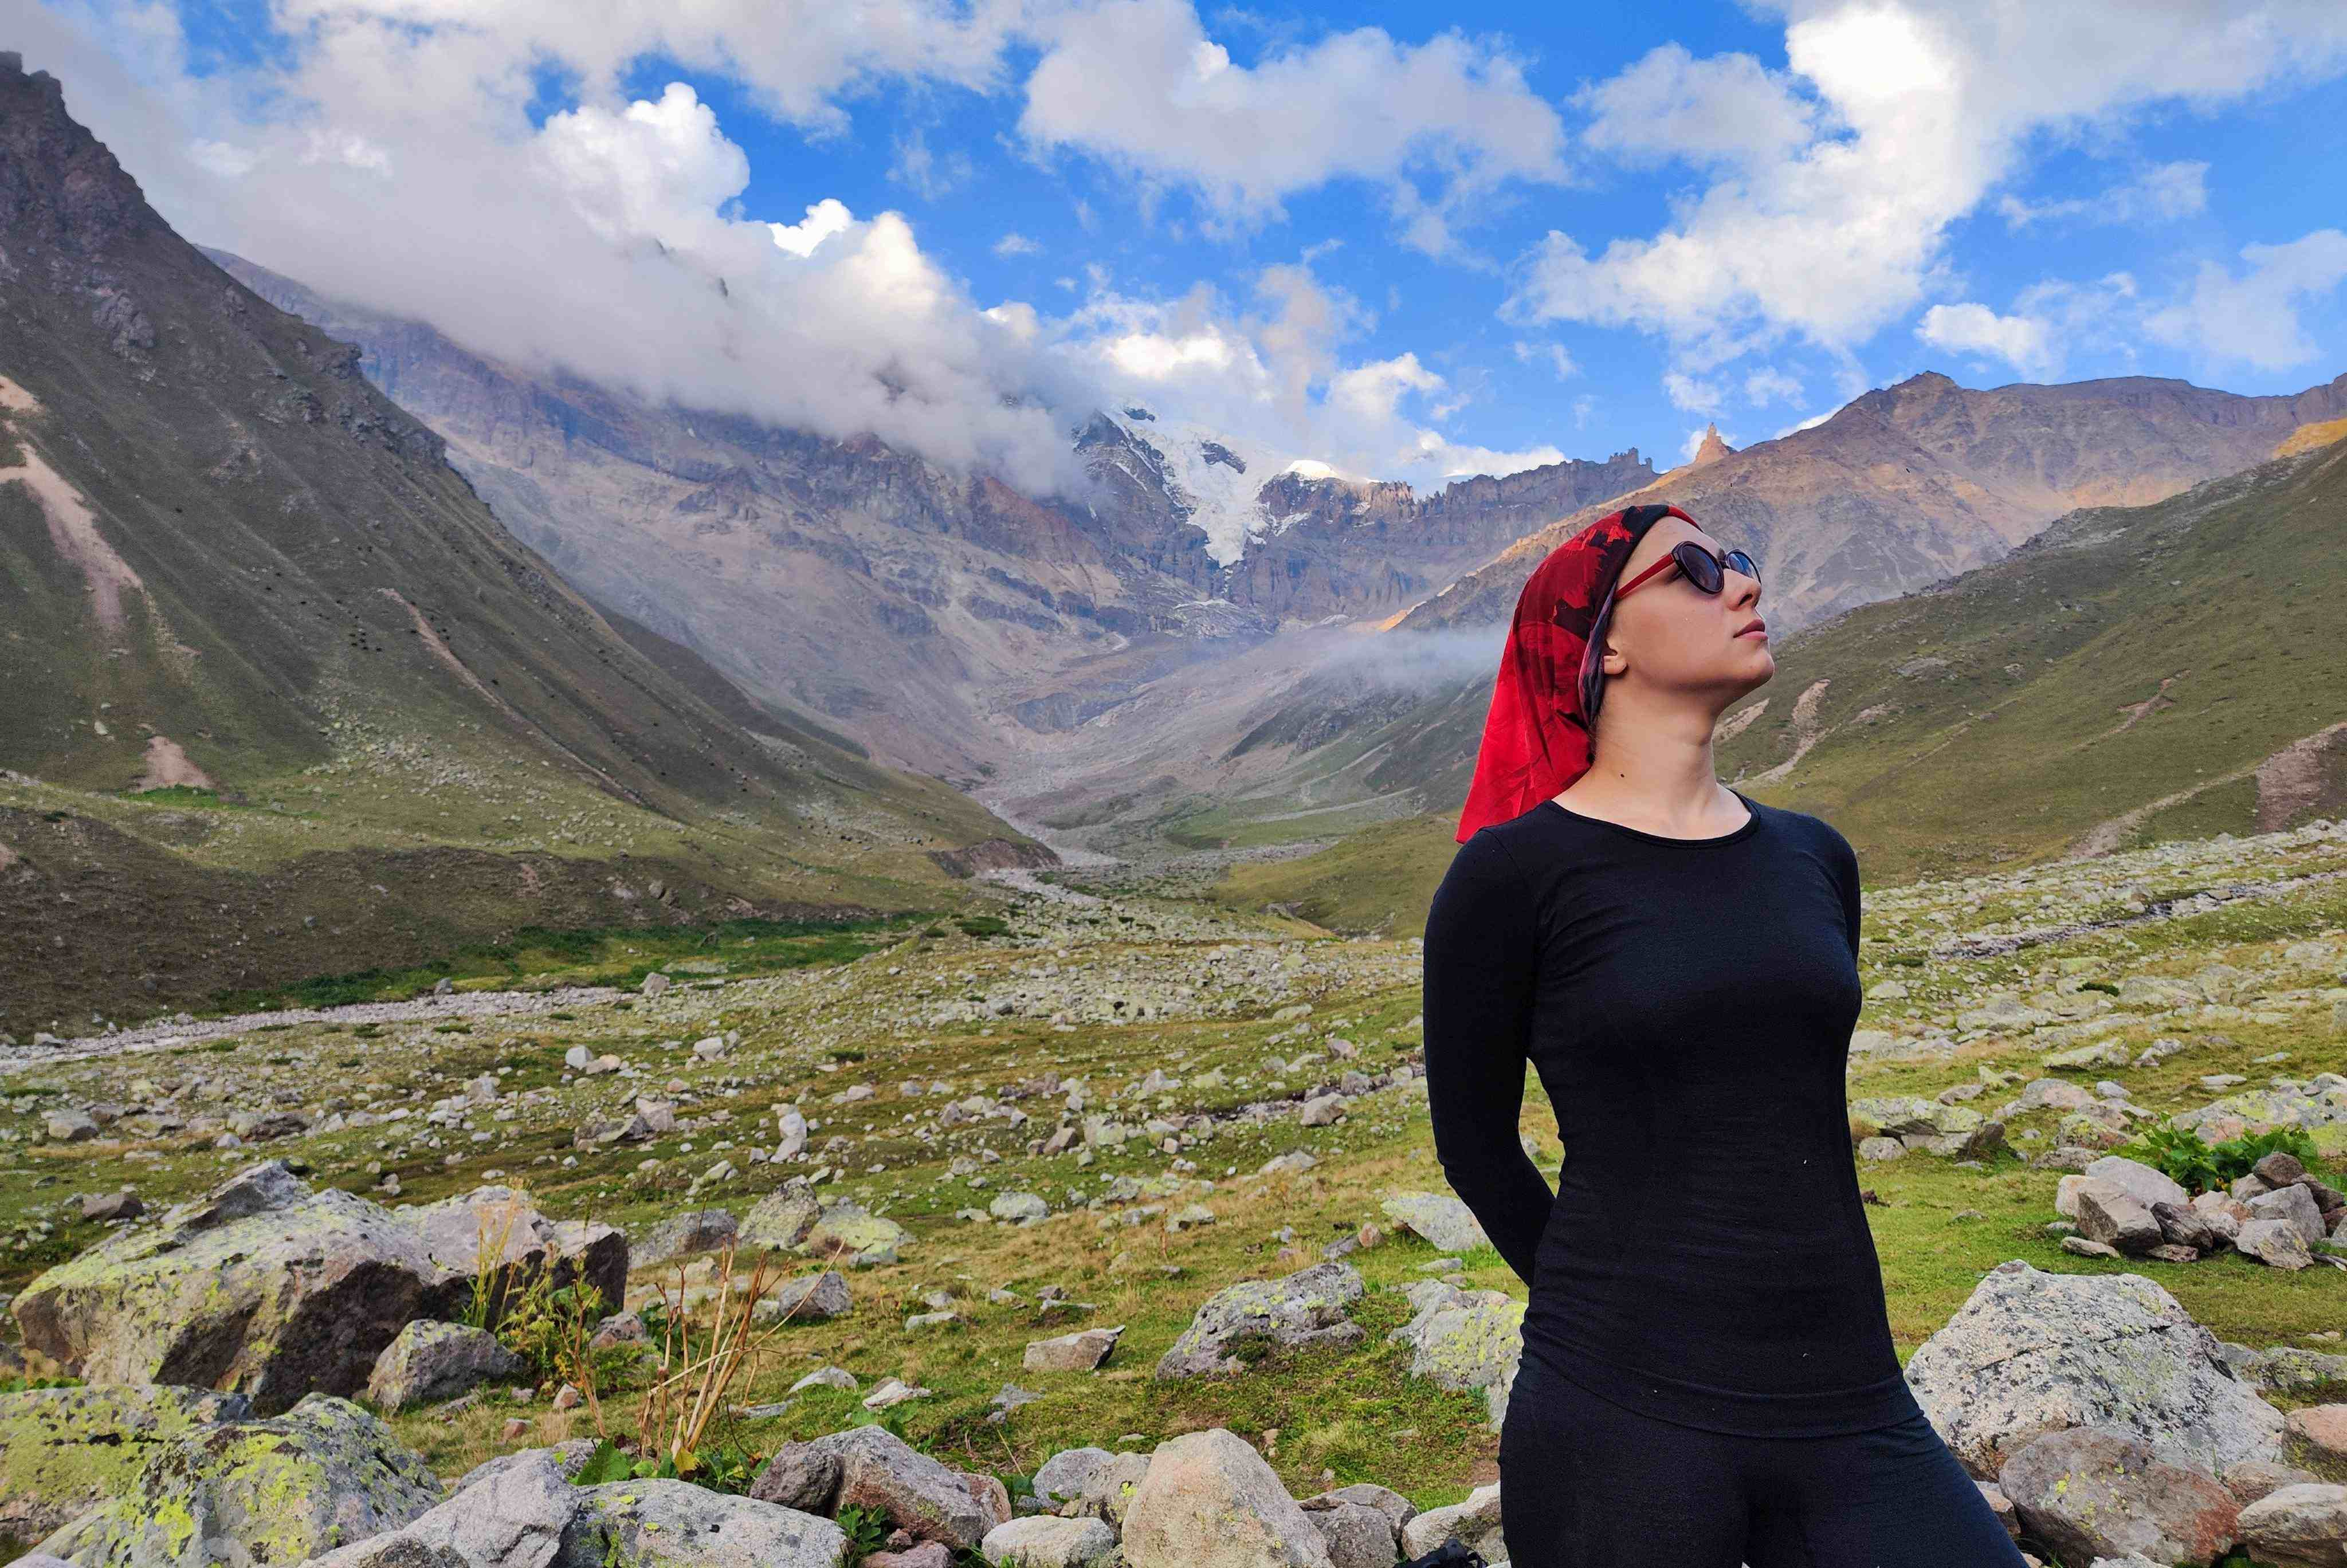
\includegraphics[width=0.7\linewidth]{../pics/IMG_20240829_181353.jpg}
	\caption{Вид на Эльбрус с м.н.}
	\label{fig:IMG_20240829_184033}
\end{figure}


\begin{figure}[h!]
	\centering
	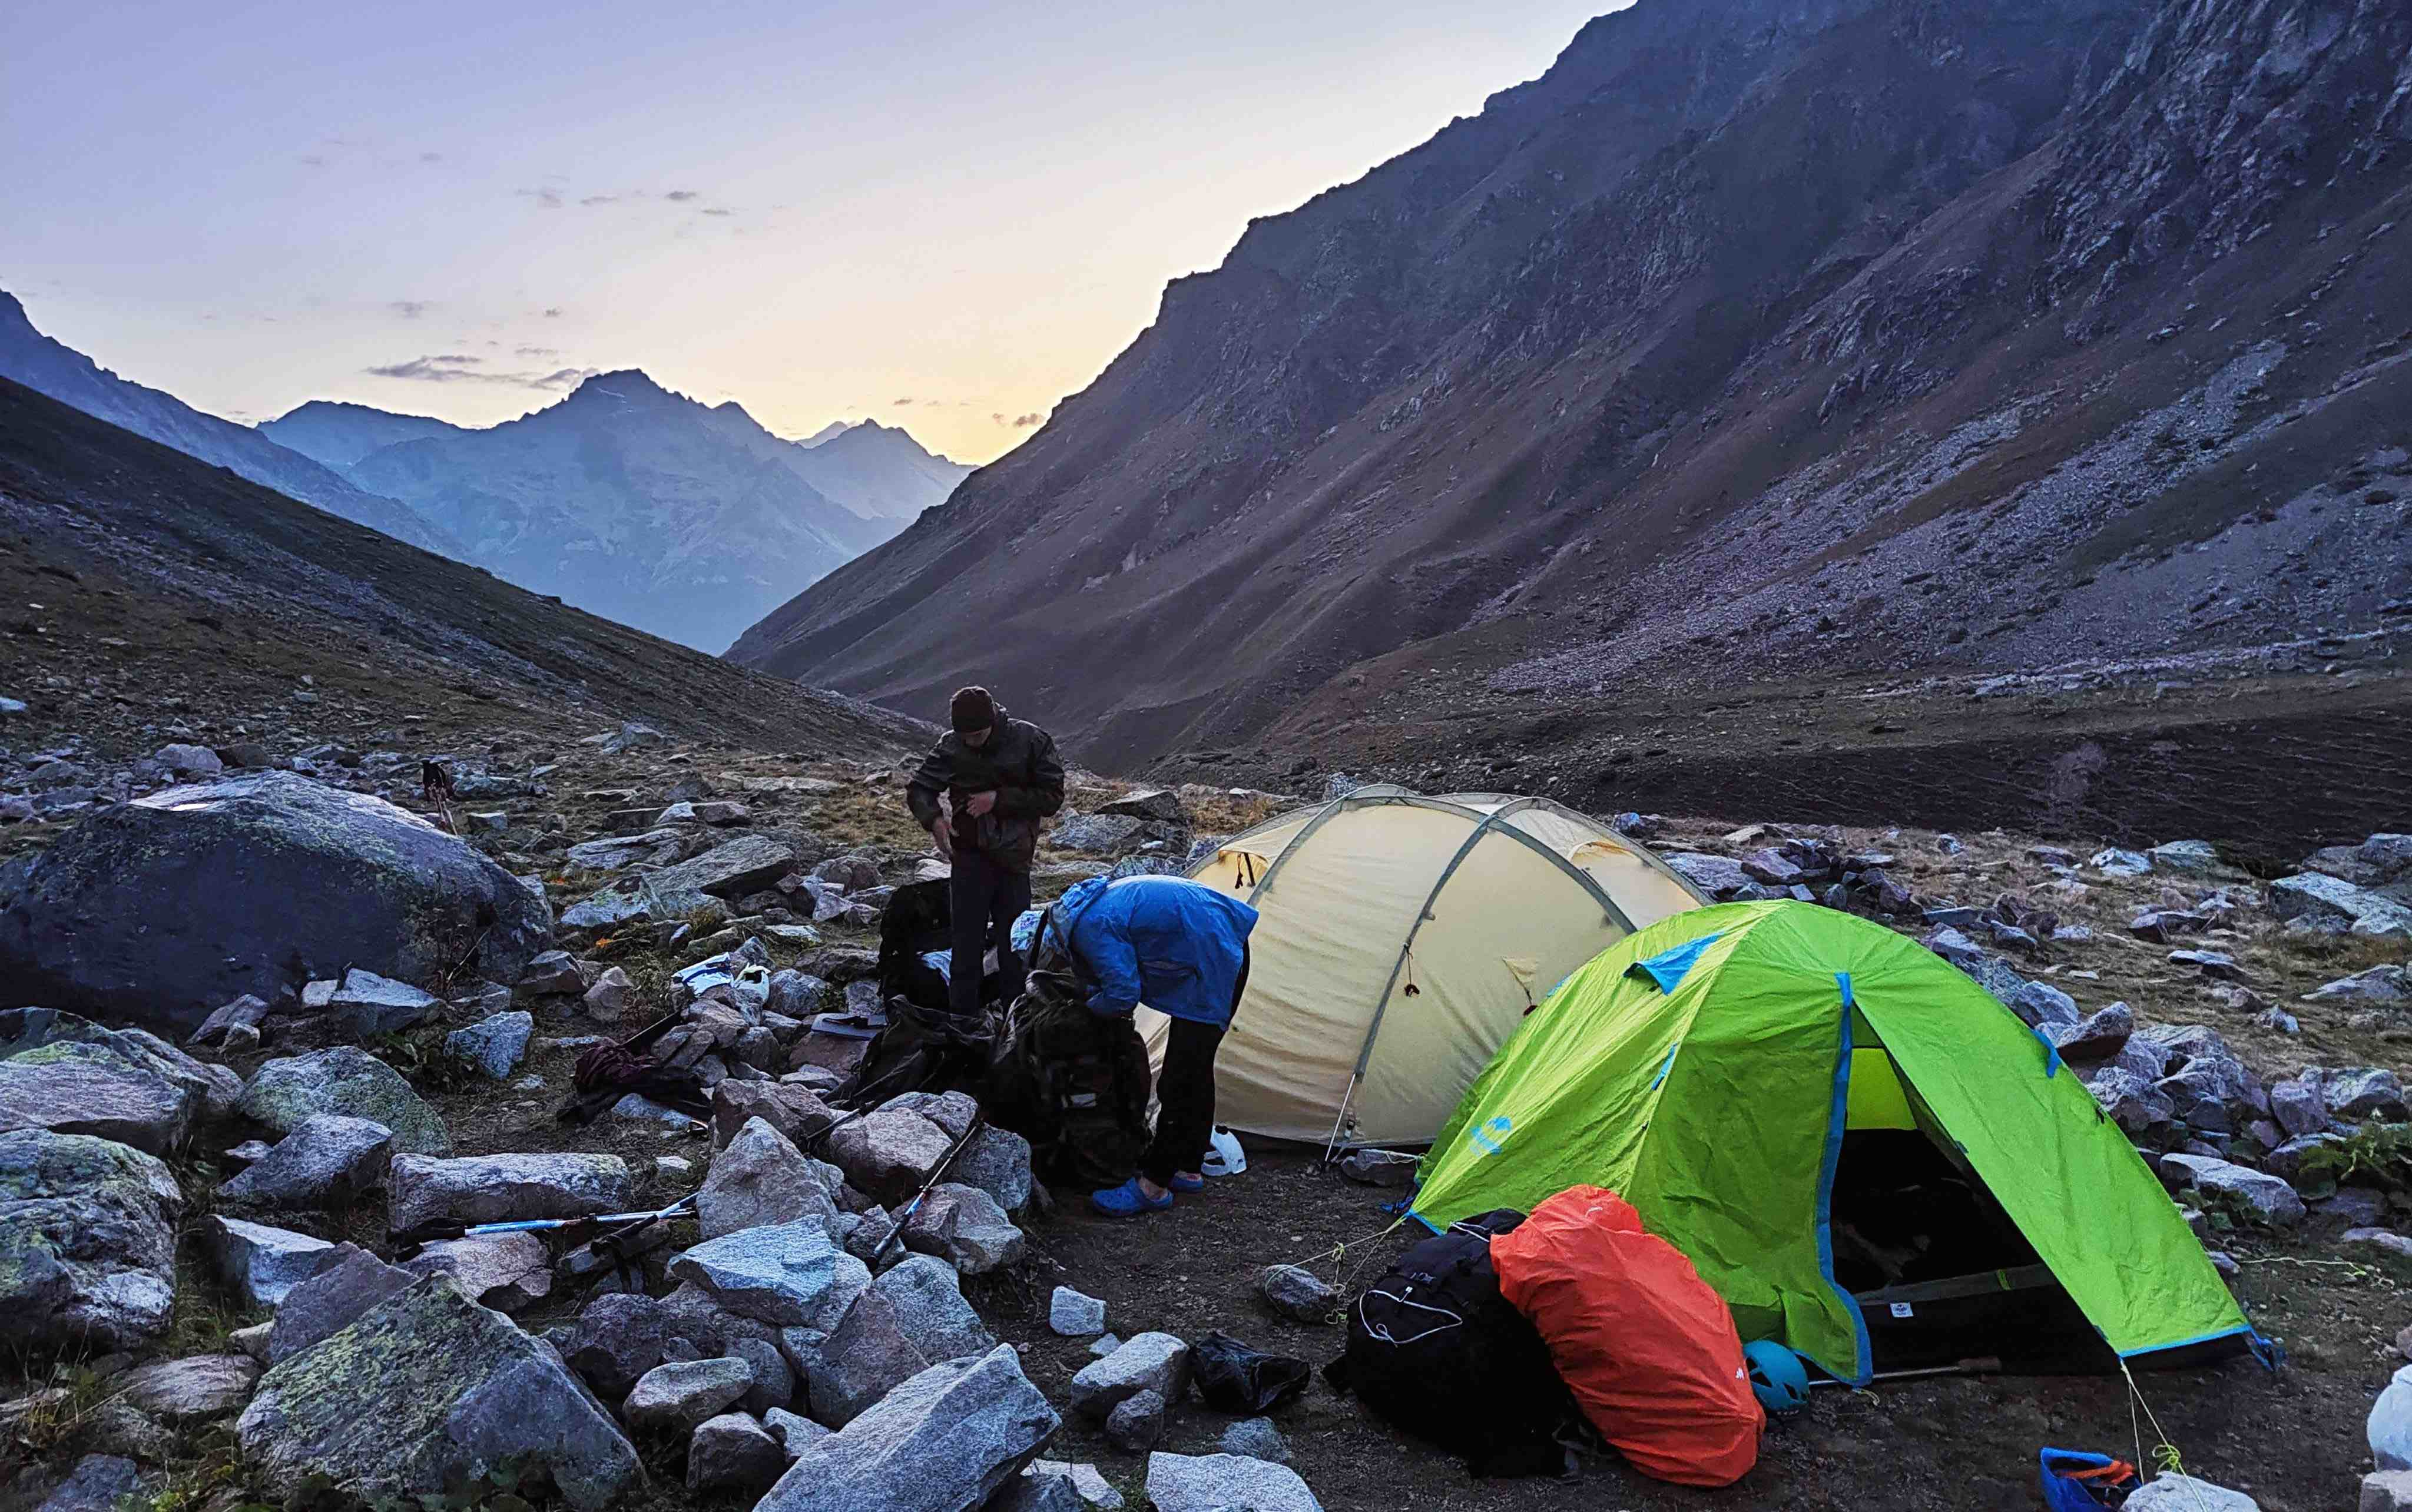
\includegraphics[width=0.7\linewidth]{../pics/IMG_20240829_191225.jpg}
	\caption{Место ночёвки 29-30 августа}
	\label{fig:IMG_20240829_191225.jpg}
\end{figure}

В 17:50 дошли до зелёных ночёвок с расчищенными площадками под палатки. На закате из-за пелены облаков на время показался Эльбрус, но оказался быстро затянут ими снова. Усилия группы окупились великолепным видом и надеждами на полное прохождение маршрута.
Координаты м.н. N43.302568\degree, E42.374594\degree.


\clearpage